%
% design.tex
%
% Copyright (C) 2022 by SpaceLab.
%
% Camera Payload Preliminary Design Review
%
% This work is licensed under the Creative Commons Attribution-ShareAlike 4.0
% International License. To view a copy of this license,
% visit http://creativecommons.org/licenses/by-sa/4.0/.
%

%
% \brief Design slides.
%
% \author Gabriel Mariano Marcelino <gabriel.mm8@gmail.com>
% \author Vitória Beatriz Bianchin <vitoriabbianchin@gmail.com>
% \author Caique Sales de Miranda Gomes <kiqsmg@gmail.com>
%
% \version 0.1.0
%
% \date 2022/06/24
%


\begin{frame}{Specifications}

    \begin{itemize}
        \item \textbf{Sensor type}: RGB
        \item \textbf{Pixel size}: 2,2 $\times$ 2,2 $\mu$m
        \item \textbf{Max. Resolution}: 1600 $\times$ 1200 px
        \item \textbf{Field of View (FoV)}: 68$^{\circ}$ (6 mm) \textcolor{red}{TBC}
        \item \textbf{Storage}: 16 MB (Flash NOR)
        \item \textbf{Power supply}: 3V3 @ 140 mA \textcolor{red}{TBC}
        \item \textbf{Interfaces}:
            \begin{itemize}
                \item \textbf{Control/Data}: SPI and/or CAN
                \item \textbf{Debug}: UART
                \item \textbf{Programming}: JTAG
            \end{itemize}
    \end{itemize}

\end{frame}

% #########################################################################
% #########################################################################

\begin{frame}{Electrical Block Diagram}

    \begin{figure}[!ht]
        \begin{center}
            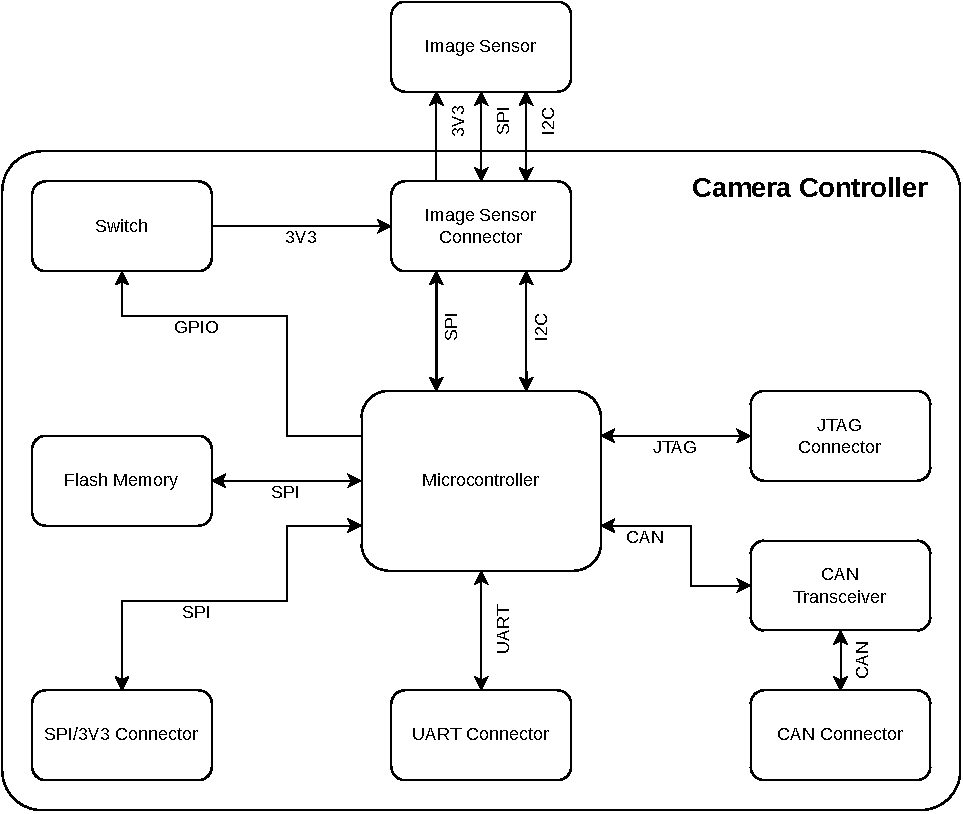
\includegraphics[scale=0.5]{figures/block-diagram}
        \end{center}
    \end{figure}

\end{frame}

% #########################################################################
% #########################################################################

\begin{frame}{Bill Of Materials}

    \begin{table}[!htb]\tiny
        \centering
        \label{tab:bom}
        \begin{tabular}{lL{2.5cm}cc}
            \toprule[1.5pt]
            \textbf{Component} & \textbf{Description} & \textbf{Partnumber} & \textbf{Quantity} \\
            \midrule
            Microcontroller        & ARM Cortex M3                & STM32F103C8T6        & 1 \\
            Flash Memory           & NOR 128 Mbit                 & W25Q128JVSIM TR      & 1 \\
            Switch                 & Load switch                  & TPS2010AD            & 1 \\
            CAN Transceiver        & CAN transceiver              & TCAN330GD            & 1 \\
            SPI/3V3 Connector      & PicoBlade 6 pin              & 532610671            & 1 \\
            UART Connector         & PicoBlade 3 pin              & 532610371            & 1 \\
            CAN Connector          & PicoBlade 3 pin              & 532610371            & 1 \\
            Image Sensor Connector & Female header 8 pin straight & -                    & 1 \\
            JTAG Connector         & Male header 4 pin angled     & -                    & 1 \\
            Image Sensor Module    & Arducam Mini 2MP Plus        & -                    & 1 \\
            Crystal                & 8 MHz crystal                & ECS-80-10-33-CHN-TR3 & 1 \\
            Lens                   & M12 lens                     & \textcolor{red}{TBD} & 1 \\
            Case                   & Aluminum case                & Custom               & 1 \\
            \bottomrule[1.5pt]
        \end{tabular}
    \end{table}

\end{frame}

% #########################################################################
% #########################################################################

\begin{frame}{Image Sensor Module}

    \begin{columns}[t]
        \begin{column}[t]{0.6\textwidth}
            \begin{itemize}
                \item Module: \href{https://www.arducam.com/product/arducam-2mp-spi-camera-b0067-arduino/}{\textcolor{blue}{\underline{Arducam Mini 2MP Plus}}}
                \item Image sensor: OV2640
                \item Sensor type: RGB CMOS
                \item Res.: 2 MP (1600 $\times$ 1200 px)
                \item Power supply: 3,3/5 V
                \item Interfaces:
                    \begin{itemize}
                        \item Control: I$^{2}$C
                        \item Data: SPI
                    \end{itemize}
                \item Lens mount: M12
                \item Dimensions: 34 $\times$ 24 mm
            \end{itemize}
        \end{column}
        \begin{column}[t]{0.4\textwidth}
            \begin{figure}[!ht]
                \begin{center}
                    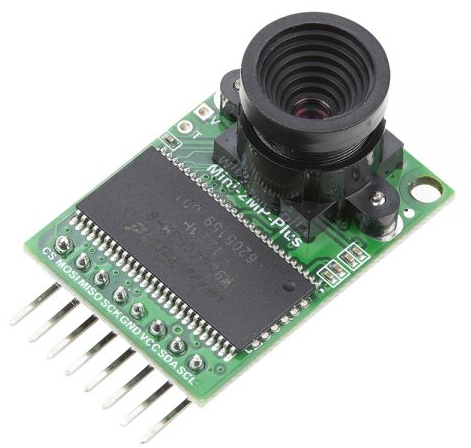
\includegraphics[width=3cm]{figures/arducam-2mp}
                \end{center}
            \end{figure}
            \begin{columns}[t]
                \begin{column}[t]{0.5\textwidth}
                    \begin{figure}[!ht]
                        \begin{center}
                            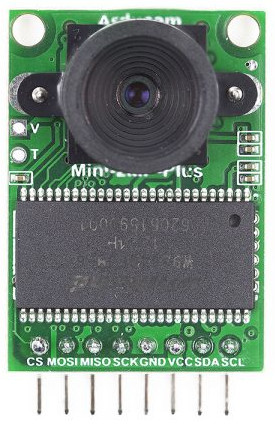
\includegraphics[width=2cm]{figures/arducam-top}
                        \end{center}
                    \end{figure}
                \end{column}
                \begin{column}[t]{0.5\textwidth}
                    \begin{figure}[!ht]
                        \begin{center}
                            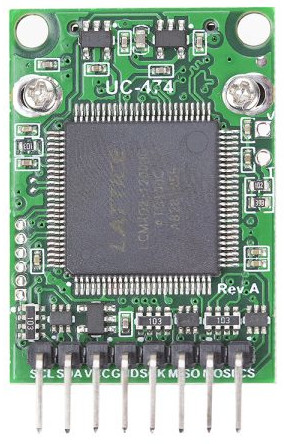
\includegraphics[width=2cm]{figures/arducam-bottom}
                        \end{center}
                    \end{figure}
                \end{column}
            \end{columns}
        \end{column}
    \end{columns}

\end{frame}

% #########################################################################
% #########################################################################

\begin{frame}{Image Sensor Module: Architecture}

    \begin{figure}[!ht]
        \begin{center}
            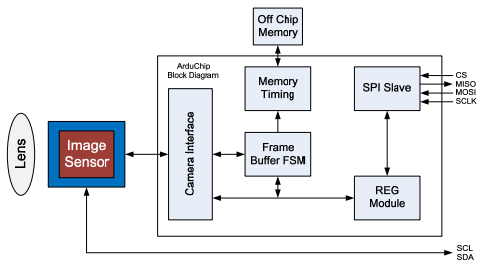
\includegraphics[width=8cm]{figures/arducam-block-diagram}
        \end{center}
    \end{figure}        
    
    \begin{itemize}
        \item ArduChip: FPGA (Lattice)
        \item Off Chip Memory: FIFO
        \item Image Sensor: OmniVision OV2640
    \end{itemize}
                        
\end{frame}             
 
% #########################################################################
% #########################################################################

\begin{frame}{Image Sensor Module: Dimensions}

    \begin{figure}[!ht]
        \begin{center}
            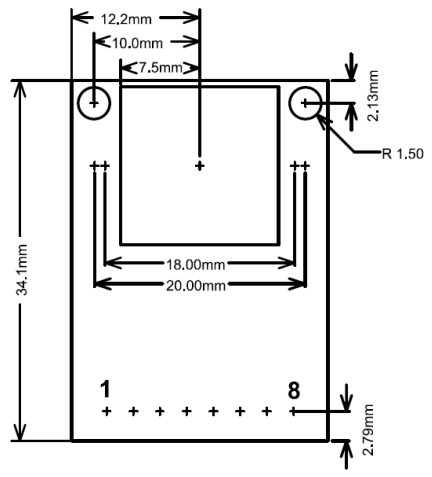
\includegraphics[width=6cm]{figures/arducam-dimensions}
        \end{center}
    \end{figure}        
    
\end{frame}             

% #########################################################################
% #########################################################################

\begin{frame}{Controller}

    \begin{columns}[t]
        \begin{column}[t]{0.5\textwidth}
            \vspace{0.2cm}
            \begin{itemize}
                \item Dimensions: 42,2 $\times$ 25,4 mm
                \vspace{0.15cm}
                \item Mounting: 4 $\times$ 3,2 mm screw holes
                \vspace{0.15cm}
                \item Connectors: Pin header and PicoBlade
                \vspace{0.15cm}
                \item Layers: 2
                \vspace{0.15cm}
                \item EDA tool: KiCad v5
                \vspace{0.15cm}
                \item Status: In progress
            \end{itemize}
        \end{column}
        \begin{column}[t]{0.6\textwidth}
            \begin{columns}[t]
                \begin{column}[t]{0.3\textwidth}
                    \begin{figure}[!ht]
                        \begin{center}
                            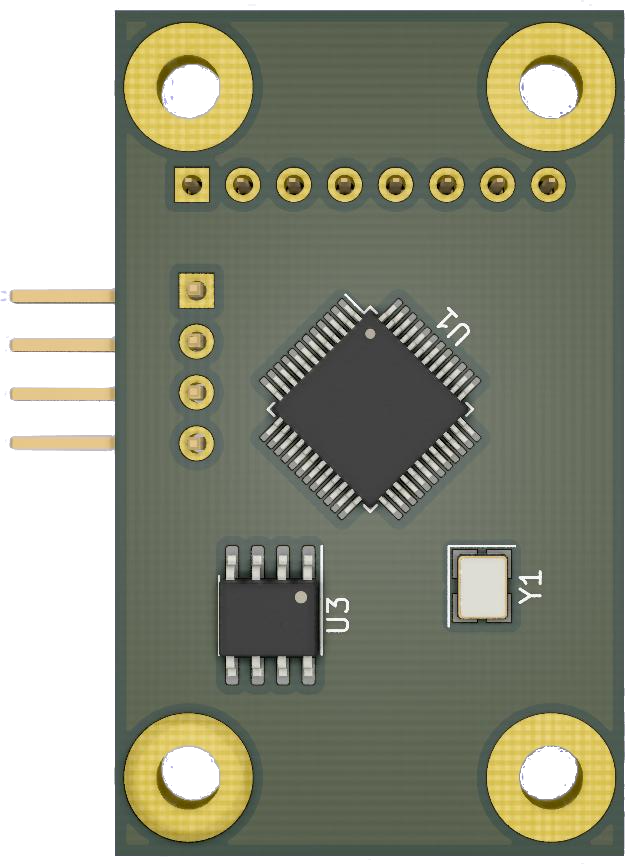
\includegraphics[height=3cm]{figures/slcam-bottom}
                        \end{center}
                    \end{figure}        
                \end{column}
                \begin{column}[t]{0.3\textwidth}
                    \begin{figure}[!ht]
                        \begin{center}
                            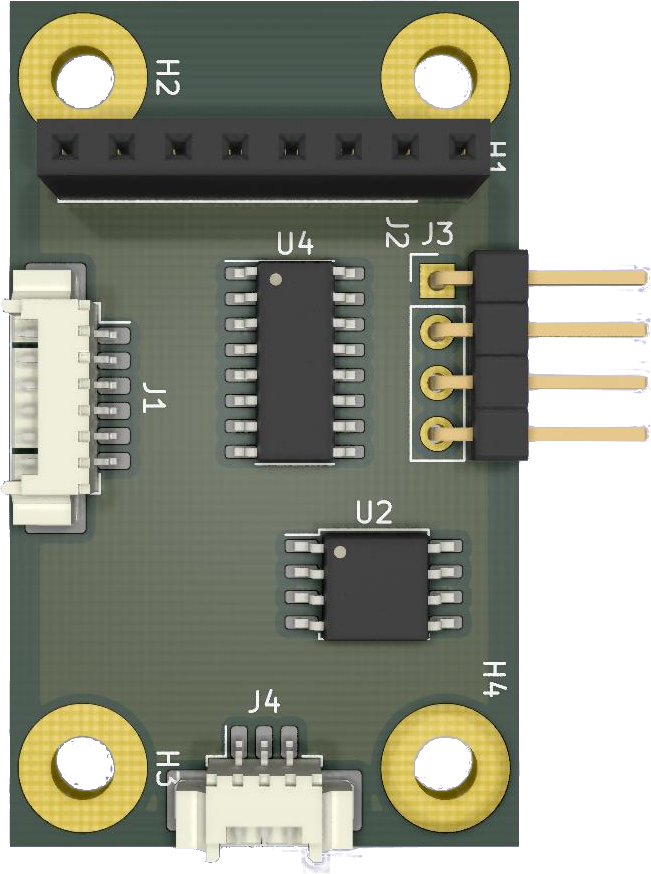
\includegraphics[height=3.07cm]{figures/slcam-top}
                        \end{center}
                    \end{figure}        
                \end{column}
            \end{columns}
            \begin{figure}[!ht]
                \begin{center}
                    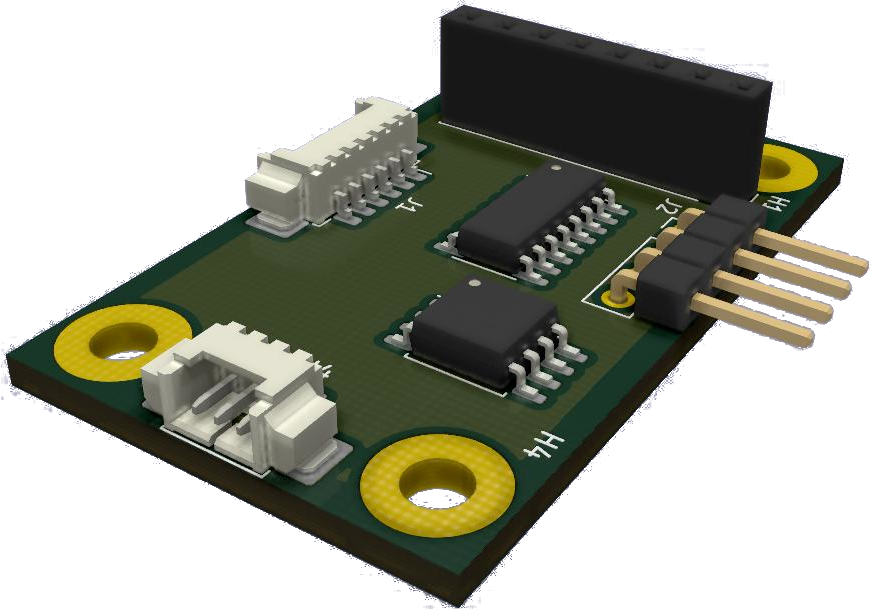
\includegraphics[width=4cm]{figures/slcam}
                \end{center}
            \end{figure}
        \end{column}
    \end{columns}

\end{frame}

% #########################################################################
% #########################################################################

\begin{frame}{Power Consumption}

    \begin{itemize}
        \item Image module\footnote{Can be turned off independently of the controller}:
            \begin{itemize}
                \item Normal mode: 350 mW
                \vspace{0.2cm}
                \item Low power mode: 100 mW
            \end{itemize}
        \vspace{0.3cm}
        \item Controller: 100 mW (estimated)
        \vspace{0.3cm}
        \item Total: 100 to 450 mW (estimated)
    \end{itemize}

\end{frame}

% #########################################################################
% #########################################################################

\begin{frame}{Electric Interfaces (ICD)}

    \begin{columns}[t]
        \begin{column}[t]{0.5\textwidth}
            \begin{itemize}
                \item Four interfaces:
                    \begin{itemize}
                        \item \textbf{SPI/Power}: Data/control and power source
                        \vspace{0.2cm}
                        \item \textbf{CAN}: Data/control
                        \vspace{0.2cm}
                        \item \textbf{UART}: Debug/log messages
                        \vspace{0.2cm}
                        \item \textbf{JTAG}: Firmware programming
                    \end{itemize}
            \end{itemize}
        \end{column}
        \begin{column}[t]{0.6\textwidth}
            \begin{table}[!htb]\tiny
                \centering
                \label{tab:icd}
                \begin{tabular}{lcl}
                    \toprule[1.5pt]
                    \textbf{Interface} & \textbf{Connector} & \textbf{Pins}\\
                    \midrule
                    \multirow{6}{*}{SPI/Power}    & \multirow{6}{*}{J1 - PicoBlade} & 3V3 \\
                                                  &                     & GND \\
                                                  &                     & MOSI \\
                                                  &                     & MISO \\
                                                  &                     & CLK \\
                                                  &                     & CS \\
                    \midrule
                    \multirow{4}{*}{JTAG}         & \multirow{4}{*}{J3 - Pin Header} & GND \\
                                                  &                     & 3V3 \\
                                                  &                     & CLK \\
                                                  &                     & DIO \\
                    \midrule
                    \multirow{3}{*}{CAN}          & \multirow{3}{*}{J4 - PicoBlade} & GND \\
                                                  &                     & CAN High \\
                                                  &                     & CAN Low \\
                    \midrule
                    \multirow{3}{*}{UART}         & \multirow{3}{*}{J5 - Pin Header} & GND \\
                                                  &                     & TX \\
                                                  &                     & RX \\
                    \bottomrule[1.5pt]
                \end{tabular}
            \end{table}
        \end{column}
    \end{columns}

\end{frame}

% #########################################################################
% #########################################################################

\begin{frame}{Optic System}

    \begin{columns}[t]
        \begin{column}[t]{0.5\textwidth}
            \vspace{1.2cm}
            \begin{itemize}
                \item Mount: S-Mount (M12)
                \vspace{0.2cm}
                \item FoV: 68$^{\circ}$ \textcolor{red}{TBC}
                \vspace{0.2cm}
                \item Focal length: 6 mm \textcolor{red}{TBC}
                \vspace{0.2cm}
                \item With IR-filter
                \vspace{0.2cm}
                \item Focus: Fixed, infinity
            \end{itemize}
        \end{column}
        \begin{column}[t]{0.5\textwidth}
            \begin{figure}[!ht]
                \begin{center}
                    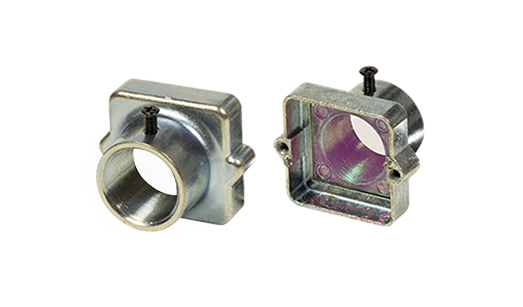
\includegraphics[width=6cm]{figures/m12-mounting.png}
                \end{center}
            \end{figure}
            \begin{figure}[!ht]
                \begin{center}
                    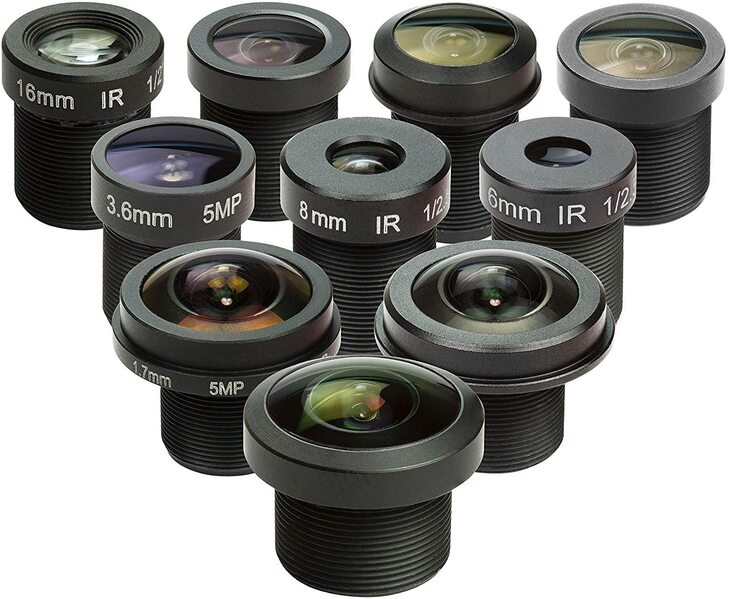
\includegraphics[width=3cm]{figures/m12-lens.jpg}
                \end{center}
            \end{figure}
        \end{column}
    \end{columns}

\end{frame}

% #########################################################################
% #########################################################################

\begin{frame}{Mechanical Structure}

    \begin{columns}[t]
        \begin{column}[t]{0.5\textwidth}
            \begin{itemize}
                \item Material: Aluminum 6061
                \vspace{0.3cm}
                \item Mass:
                    \begin{itemize}
                        \item Image module: 20 g
                        \vspace{0.2cm}
                        \item Controller: $\cong$ 10 g
                        \vspace{0.2cm}
                        \item Case: $\cong$ 22,4 g
                        \vspace{0.2cm}
                        \item Total: \textbf{52,4 g}
                    \end{itemize}
                \vspace{0.3cm}
                \item Fabrication: CNC miling
            \end{itemize}
        \end{column}
        \begin{column}[t]{0.5\textwidth}
        \vspace{0.5cm}
            \begin{figure}[!ht]
                \begin{center}
                    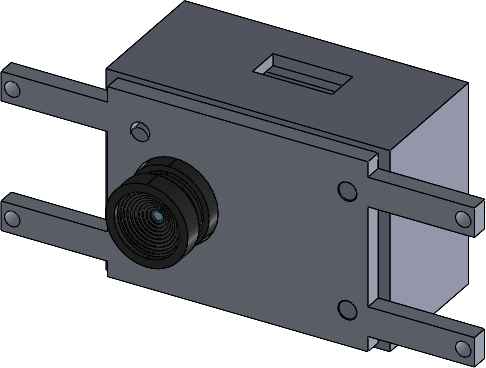
\includegraphics[width=4cm]{figures/slcam-overview.png}
                \end{center}
            \end{figure}
        \end{column}
    \end{columns}

\end{frame}

\begin{frame}{Dimensions}

    \begin{figure}[!ht]
        \begin{center}
            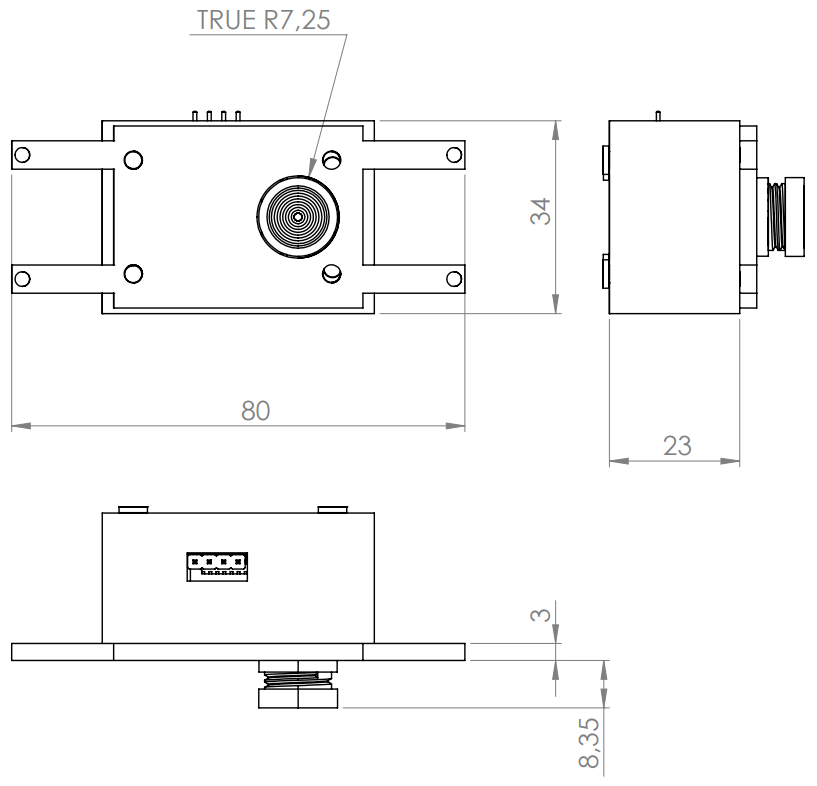
\includegraphics[width=7.5cm]{figures/slcam-drawing.png}
        \end{center}
    \end{figure}

\end{frame}

% #########################################################################
% #########################################################################

\begin{frame}{Overview}

    \begin{figure}[!ht]
        \begin{center}
            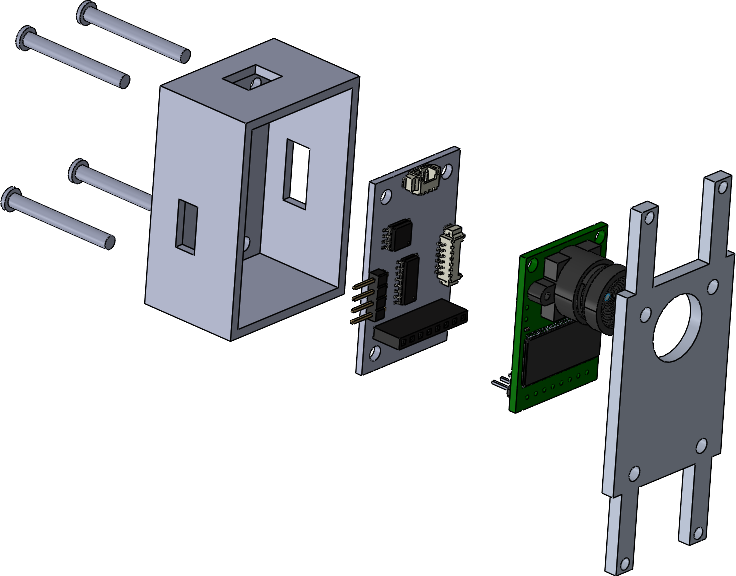
\includegraphics[width=8.5cm]{figures/slcam-exp.png}
        \end{center}
    \end{figure}

\end{frame}

% #########################################################################
% #########################################################################

\begin{frame}{Satellite Integration: 2U Structure}

    \begin{columns}[t]
        \begin{column}[t]{0.3\textwidth}
            \begin{figure}[!ht]
                \begin{center}
                    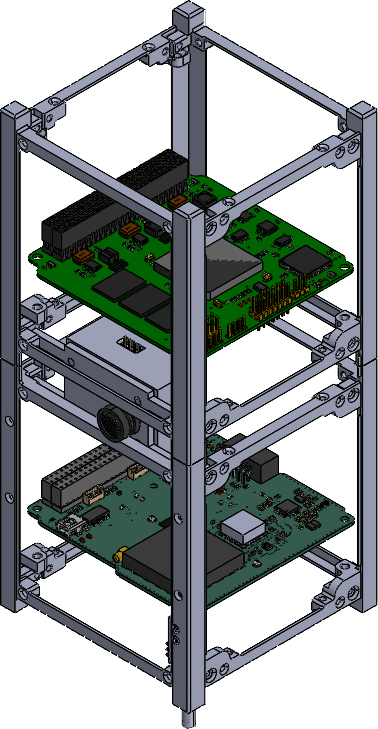
\includegraphics[width=3cm]{figures/slcam-ex1.png}
                \end{center}
            \end{figure}
        \end{column}
        \begin{column}[t]{0.3\textwidth}
            \begin{figure}[!ht]
                \begin{center}
                    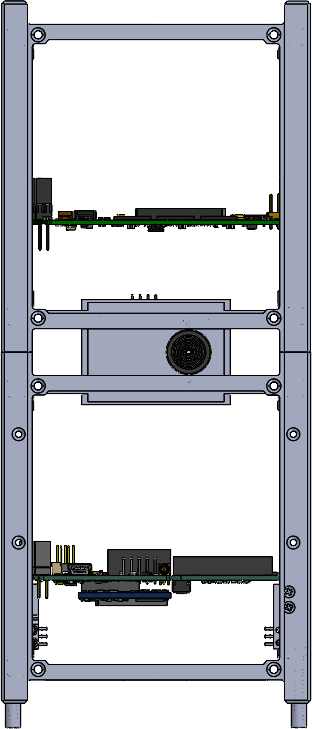
\includegraphics[width=2.7cm]{figures/slcam-ex2.png}
                \end{center}
            \end{figure}
        \end{column}
        \begin{column}[t]{0.3\textwidth}
            \begin{figure}[!ht]
                \begin{center}
                    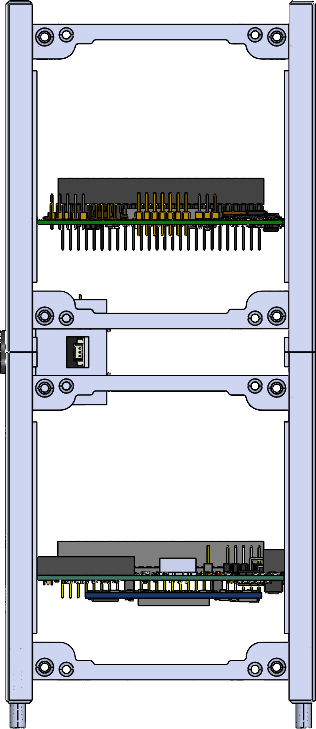
\includegraphics[width=2.7cm]{figures/slcam-ex3.png}
                \end{center}
            \end{figure}
        \end{column}
    \end{columns}

\end{frame}

% #########################################################################
% #########################################################################

\begin{frame}{Firmware}

    \begin{itemize}
        \item Language: C
        \vspace{0.3cm}
        \item OS: FreeRTOS
        \vspace{0.3cm}
        \item Layers:
            \begin{itemize}
                \item HAL
                \vspace{0.2cm}
                \item Drivers
                \vspace{0.2cm}
                \item Devices
                \vspace{0.2cm}
                \item Tasks
                \vspace{0.2cm}
                \item Libraries
                \vspace{0.2cm}
                \item System
            \end{itemize}
    \end{itemize}

\end{frame}

% #########################################################################
% #########################################################################

\begin{frame}{Firmware: Development Environment}

    \begin{columns}[t]
        \begin{column}[t]{0.6\textwidth}
            \begin{itemize}
                \vspace{0.4cm}
                \item Hardware: Generic STM32 Cortex-M3 dev kit
                \vspace{0.4cm}
                \item Programmer: ST-Link V2
                \vspace{0.4cm}
                \item Compiler: GCC (arm-none-eabi-XXX)
                \vspace{0.4cm}
                \item Programming tool: \href{https://github.com/stlink-org/stlink}{\textcolor{blue}{\underline{stlink}}}
            \end{itemize}
        \end{column}
        \begin{column}[t]{0.4\textwidth}
            \begin{figure}[!ht]
                \begin{center}
                    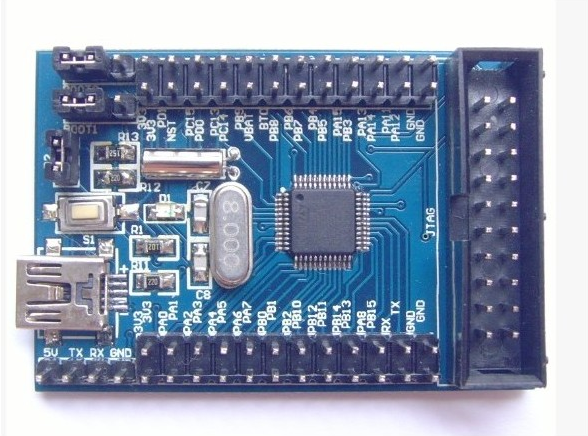
\includegraphics[width=4cm]{figures/stm32-dev-kit}
                \end{center}
            \end{figure}
            \begin{figure}[!ht]
                \begin{center}
                    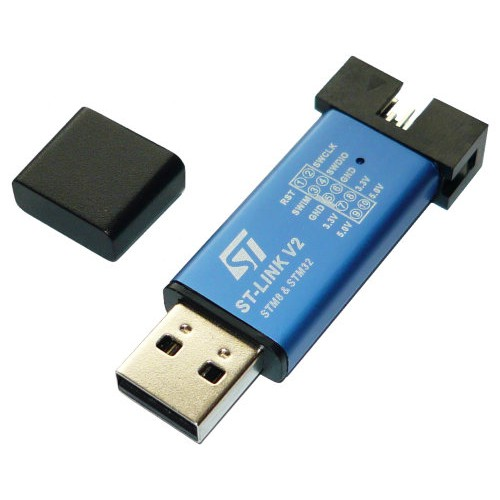
\includegraphics[width=3.5cm]{figures/stlink-v2}
                \end{center}
            \end{figure}
        \end{column}
    \end{columns}
\end{frame}

% #########################################################################
% #########################################################################

\begin{frame}{Firmware: Verification \& Validation}

    \begin{itemize}
        \item Unit tests: \href{https://cmocka.org/}{\textcolor{blue}{\underline{CMocka}}}
        \vspace{0.5cm}
        \item Static analysis: \href{https://cppcheck.sourceforge.io/}{\textcolor{blue}{\underline{CppCheck}}}
        \vspace{0.5cm}
        \item Code style: \href{https://www.misra.org.uk/}{\textcolor{blue}{\underline{MISRA-C 2012}}}
    \end{itemize}

\end{frame}

% #########################################################################
% #########################################################################

\begin{frame}{Firmware: Commands}

\begin{table}[!htb]
    \centering
    \label{tab:commands}
    \begin{tabular}{cll}
        \toprule[1.5pt]
        \textbf{ID} & \textbf{Command} & \textbf{Parameters}\\
        \midrule
        1 & Read ID                 & None \\
        2 & Power On/Off sensor     & 1 or 0 \\
        3 & Take picture            & None \\
        4 & Enable periodic capture & None \\
        5 & Read last picture       & None \\
        6 & Delete last picture     & None \\
        7 & Erase memory            & None \\
        8 & Set parameter           & Parameter ID + Parameter value \\
        9 & Get parameter           & Parameter ID \\
        \bottomrule[1.5pt]
    \end{tabular}
\end{table}

\end{frame}

\begin{frame}{Firmware: Parameters}

\begin{table}[!htb]
    \centering
    \label{tab:parameters}
    \begin{tabular}{cllc}
        \toprule[1.5pt]
        \textbf{ID} & \textbf{Name} & \textbf{Type} & \textbf{Access} \\
        \midrule
        0 & Module ID                   & uint16 & R\\
        1 & Sensor status               & uint8  & R  \\
        2 & Capture period (in seconds) & uint8  & R/W \\
        4 & Pictures in memory          & uint8  & R \\
        \bottomrule[1.5pt]
    \end{tabular}
\end{table}

\end{frame}

% #########################################################################
% #########################################################################

\begin{frame}{Software}

    \begin{columns}[t]
        \begin{column}[t]{0.55\textwidth}
            \begin{itemize}
                \item Software for test/validade the camera module
                \item Purpose:
                    \begin{itemize}
                        \item Send commands to the camera
                        \item Read the images from the camera
                    \end{itemize}
                \item Language: Python
                \item Communication between PC and camera: USB/SPI or USB/CAN converter
            \end{itemize}
        \end{column}
        \begin{column}[t]{0.45\textwidth}
            \vspace{0.5cm}
            \begin{figure}[!ht]
                \begin{center}
                    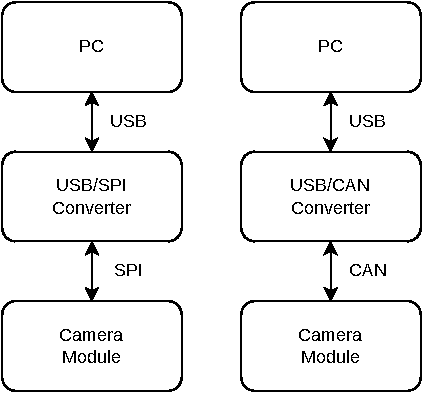
\includegraphics[width=4.5cm]{figures/software-diagram}
                \end{center}
            \end{figure}
        \end{column}
    \end{columns}

\end{frame}